\documentclass[11pt,letterpaper]{article}
\usepackage{fontspec}
\usepackage[spanish,es-noshorthands,es-tabla,es-lcroman]{babel}
\usepackage{plantilla/unab_reporte}

% Los datos compartidos se generan desde datos.md al ejecutar compilar.py.
\input{.build/datos.tex}
\hypersetup{pdftitle={\TituloTrabajo},pdfauthor={\Grupo}}

\begin{document}
\portadareporte
\pagenumbering{roman}
\tableofcontents
\clearpage
\pagenumbering{arabic}
\setcounter{section}{1} % La portada es el apartado 1


% ==============================================================================
% ¡ATENCIÓN! ESTIPULACIÓN IMPORTANTE DEL USUARIO:
% POR NINGÚN MOTIVO SE DEBE MODIFICAR LA PORTADA, TÍTULO, PLANTEAMIENTO DEL PROBLEMA,
% JUSTIFICACIÓN, NI LOS OBJETIVOS DE LA INVESTIGACIÓN. ESTAS SECCIONES SON DEFINITIVAS.
% ==============================================================================
\section{Título de la investigación}
\TituloTrabajo

\section{Introducción}

\section{Planteamiento del problema}
\subsection{Situación problemática}
Las sedes de soporte técnico e infraestructura digital del sector educativo
manejan volúmenes significativos de tráfico y equipos con diferentes niveles de
confianza. En la sede interactúan estaciones del personal de planta con laptops
y tabletas estudiantiles que ingresan para mantenimiento. La arquitectura actual
es predominantemente plana y no existe una separación lógica formal entre los
dominios técnico y administrativo. Equipos en revisión, potencialmente
desactualizados o infectados con malware, comparten el canal con sistemas que
procesan registros institucionales.

La red carece de ACL estrictas, inspección de estado mediante cortafuegos
dedicados, NAT estructurado por zonas y filtrado en capa de aplicación. Tampoco
se dispone de políticas formales para el uso seguro de puertos y servicios. Esta
carencia eleva la probabilidad de denegación de servicio interna, fugas de
información, accesos no autorizados e interrupciones en la entrega de equipos.

\subsection{Enunciado del problema}
¿De qué manera el diseño de un modelo de seguridad perimetral y segmentación
lógica contribuirá a mitigar los riesgos informáticos y garantizar la
confidencialidad, integridad y disponibilidad en la red de datos de la Sede de
Enlaces con la Educación en Santa Rosa de Lima durante 2026?

\section{Justificación}
La investigación responde a la necesidad de dotar a la sede de un esquema de
seguridad formal, preventivo y técnicamente viable. La propuesta aborda las
vulnerabilidades estructurales mediante VLAN para aislar dispositivos en
diagnóstico, estaciones administrativas y servidores locales; reglas de
filtrado perimetral en Linux; y servicios proxy para auditar el tráfico y
optimizar el ancho de banda. En el ámbito académico y profesional, permite
aplicar competencias de seguridad de redes, gestión de riesgos, simulación en
GNS3 y normativa informática salvadoreña. El resultado esperado es una base
documental replicable en otras sedes regionales.

\section{Objetivos de la investigación}
\subsection{Objetivo general}
Diseñar un modelo de seguridad perimetral y segmentación lógica para la red de
datos de la Sede de Enlaces con la Educación en el distrito de Santa Rosa de
Lima, con el fin de mitigar riesgos informáticos y preservar la
confidencialidad, integridad y disponibilidad del tráfico institucional durante
2026.
\subsection{Objetivos específicos}
\begin{itemize}
  \item Diagnosticar las condiciones técnicas actuales de la infraestructura,
  estaciones y flujos de tráfico, identificando vulnerabilidades y amenazas.
  \item Formular una matriz de análisis y evaluación de riesgos y Políticas de
  Seguridad Informática alineadas al marco regulatorio y operativo institucional.
  \item Estructurar en GNS3 una arquitectura perimetral con VLAN, ACL y
  cortafuegos Linux para aislar zonas administrativas, técnicas y de diagnóstico.
  \item Configurar controles de capa de aplicación mediante proxy y certificados
  digitales HTTPS/TLS en un laboratorio simulado.
\end{itemize}


% ==============================================================================
% FIN DE SECCIONES PROTEGIDAS Y DEFINITIVAS
% ==============================================================================
\section{Marco teórico}

El desarrollo de una propuesta de seguridad para una red de datos requiere comprender los fundamentos relacionados con la seguridad informática, la seguridad de redes, la segmentación lógica y los mecanismos utilizados para controlar el intercambio de información entre dispositivos. Estos elementos permiten analizar las condiciones de una infraestructura tecnológica y establecer medidas orientadas a disminuir los riesgos asociados con accesos no autorizados, propagación de amenazas y exposición de información.

En el caso de la Sede de Enlaces con la Educación del distrito de Santa Rosa de Lima, la importancia de estos fundamentos se relaciona directamente con las condiciones actuales de su infraestructura. La sede dispone de una sola red en la que se conectan los equipos utilizados por el personal y mantiene una topología de tipo estrella. Por esta razón, resulta necesario estudiar los conceptos técnicos que fundamentan el diseño de un modelo de seguridad perimetral y segmentación lógica adecuado a las características de dicha red.

\subsection{Seguridad informática}

La seguridad informática comprende el conjunto de principios, medidas, procedimientos y controles destinados a proteger los sistemas de información, dispositivos, redes y datos frente a amenazas que puedan afectar su funcionamiento o permitir el acceso, modificación, destrucción o divulgación no autorizada de la información.

Dentro de la seguridad de la información, tres propiedades constituyen una referencia fundamental: confidencialidad, integridad y disponibilidad. La confidencialidad busca que la información únicamente pueda ser conocida o utilizada por personas, sistemas o procesos autorizados; la integridad procura mantener la exactitud y consistencia de la información, evitando alteraciones no autorizadas; mientras que la disponibilidad pretende garantizar que los sistemas, servicios y datos puedan ser utilizados cuando sean requeridos por los usuarios autorizados.

Estos principios resultan relevantes para una infraestructura de red ya que en este tipo de redes los dispositivos intercambian información y utilizan recursos compartidos. Una deficiencia en los controles de seguridad puede facilitar accesos indebidos, interrupciones de los servicios o propagación de amenazas entre dispositivos.

En consecuencia, la seguridad informática no depende únicamente de herramientas tecnológicas. También requiere identificar los activos que deben protegerse, las amenazas existentes, las vulnerabilidades que pueden ser aprovechadas y los riesgos derivados de la combinación de estos factores. A partir de dicho análisis es posible establecer controles acordes con las necesidades y características de una organización.

\subsection{Seguridad de redes}

La seguridad de redes constituye una aplicación de los principios de seguridad informática orientada específicamente a proteger la infraestructura de comunicaciones, los dispositivos conectados y el tráfico que circula entre ellos. Su finalidad es establecer mecanismos que permitan controlar las comunicaciones y reducir la posibilidad de accesos o intercambios de información no autorizados.

La protección de una red puede implementarse mediante diferentes controles, entre ellos cortafuegos, listas de control de acceso, segmentación de red, autenticación, monitoreo del tráfico y establecimiento de políticas para determinar qué dispositivos pueden comunicarse entre sí.

La seguridad de redes adquiere especial importancia cuando dispositivos con funciones o niveles de confianza diferentes utilizan una misma infraestructura. Una red sin separación suficiente entre grupos de dispositivos puede incrementar la exposición de los recursos ante incidentes originados en otro equipo conectado.

En este sentido, organismos especializados en ciberseguridad recomiendan implementar segmentación mediante mecanismos como VLAN, listas de control de acceso en routers y capacidades de firewall como parte de una estrategia de defensa en profundidad.

\subsection{Seguridad perimetral}

La seguridad perimetral comprende los mecanismos destinados a controlar las comunicaciones entre diferentes zonas de una red y entre la infraestructura interna y redes externas. El perímetro representa un punto de control desde el cual pueden establecerse reglas para permitir, restringir, inspeccionar o registrar las comunicaciones.

Uno de los principales componentes utilizados para establecer este control es el firewall o cortafuegos. Este dispositivo o software analiza el tráfico de red de acuerdo con reglas previamente establecidas y determina qué comunicaciones se permiten o se bloquean. Dependiendo de su implementación, puede realizar inspección del tráfico considerando direcciones IP, puertos, protocolos, conexiones y otros parámetros.

El diseño de un perímetro de seguridad no debe entenderse exclusivamente como una barrera entre Internet y la red interna. En arquitecturas segmentadas también pueden establecerse controles entre diferentes zonas internas, de manera que el acceso de un segmento a otro se encuentre sujeto a políticas específicas.

Para la presente investigación, este concepto constituye uno de los fundamentos de la arquitectura propuesta, puesto que el propósito es establecer controles que permitan regular el tráfico entre los diferentes grupos de dispositivos que forman parte de la infraestructura de la sede.

\subsection{Segmentación lógica de redes}

La segmentación de redes consiste en dividir una infraestructura en diferentes segmentos con el propósito de establecer límites de comunicación y facilitar la aplicación de políticas de seguridad. Esta separación puede realizarse físicamente mediante equipos independientes o lógicamente mediante tecnologías de red.



CISA define la segmentación como una aproximación arquitectónica física o virtual mediante la cual una red es dividida en múltiples segmentos que funcionan como subredes independientes, proporcionando mayor control sobre las comunicaciones.

Una de las tecnologías empleadas para realizar esta separación lógica son las Virtual Local Area Networks (VLAN). Las VLAN permiten agrupar dispositivos lógicamente aunque utilicen una infraestructura física común. De esta manera, los equipos pueden organizarse de acuerdo con su función, nivel de confianza o requerimientos de seguridad.

NIST señala que, en un enfoque tradicional de segmentación, los recursos que poseen requerimientos de seguridad similares pueden agruparse en segmentos mediante mecanismos como identificadores VLAN, mientras las políticas de comunicación se establecen utilizando parámetros de red como direcciones IP y puertos.

La utilización de VLAN permite disminuir la comunicación directa e innecesaria entre grupos de dispositivos. Sin embargo, la segmentación por sí sola no constituye un mecanismo completo de protección; debe complementarse con reglas que determinen qué tráfico puede circular entre los diferentes segmentos.

\subsection{Listas de control de acceso (ACL)}

Las listas de control de acceso, conocidas como ACL por sus siglas en inglés (Access Control Lists), permiten establecer reglas para autorizar o denegar determinados tipos de tráfico de red.

Las ACL pueden utilizar criterios como direcciones IP de origen y destino, protocolos y puertos para determinar si una comunicación debe permitirse. De esta manera, permiten aplicar restricciones entre diferentes segmentos de una infraestructura.

En una arquitectura segmentada, las ACL complementan el uso de VLAN ya que facilitan el control de la comunicación entre ellas. Esto posibilita establecer, por ejemplo, que un determinado segmento tenga acceso únicamente a los servicios necesarios para desarrollar sus funciones, evitando comunicaciones que no hayan sido expresamente autorizadas.

La aplicación de estos controles responde al principio de reducir las comunicaciones innecesarias entre grupos de dispositivos. CISA incluye las ACL de router junto con los firewalls y las VLAN entre los mecanismos que pueden utilizarse para conseguir una segmentación robusta de la red.



\subsection{Cortafuegos y filtrado del tráfico}

Un firewall constituye un mecanismo de seguridad encargado de controlar el tráfico que atraviesa diferentes interfaces o zonas de una red. Su funcionamiento se basa en políticas y reglas mediante las cuales se determina qué comunicaciones pueden establecerse y cuáles deben ser rechazadas.

Los cortafuegos pueden utilizarse tanto para controlar las conexiones procedentes de redes externas como para establecer restricciones entre segmentos internos. En una arquitectura de seguridad por capas, estos controles permiten crear fronteras entre recursos que presentan diferentes niveles de confianza.

CISA señala que los firewalls pueden configurarse para bloquear tráfico proveniente de determinadas direcciones de red, aplicaciones o puertos, permitiendo simultáneamente las comunicaciones que resultan necesarias para el funcionamiento de los servicios.

Para el modelo propuesto en esta investigación se considera el empleo de un cortafuegos basado en Linux dentro del ambiente simulado, con el propósito de establecer reglas de filtrado y controlar las comunicaciones entre los segmentos definidos.

\subsection{Proxy y control de acceso a servicios de Internet}

Un servidor proxy funciona como intermediario entre los dispositivos de una red y determinados servicios externos. Las solicitudes realizadas por los usuarios pueden ser procesadas por el proxy antes de establecer comunicación con el recurso solicitado.

Su implementación puede utilizarse para establecer políticas de navegación, controlar determinados tipos de solicitudes, mantener registros de actividad y aplicar restricciones de acceso de acuerdo con las necesidades de una organización.

Este elemento posee además un antecedente directo dentro de la infraestructura objeto de estudio. De acuerdo con la información proporcionada por la sede, anteriormente existía un servidor central encargado de filtrar y distribuir el acceso a Internet y se utilizaba un proxy físico para realizar funciones de filtrado. Con modificaciones realizadas posteriormente a la infraestructura, tanto el servidor como el proxy dejaron de utilizarse, permaneciendo principalmente el switch y el cableado de la red.

Por tanto, estudiar la función del proxy permite comprender tanto parte de la arquitectura que existió anteriormente como las posibilidades de incorporar controles de capa de aplicación dentro del modelo propuesto.



\subsection{HTTPS/TLS y protección de las comunicaciones}

La seguridad de una red no solamente requiere controlar qué dispositivos pueden establecer comunicación, sino también proteger la información mientras es transmitida. Para ello pueden utilizarse protocolos criptográficos destinados a proporcionar seguridad a las comunicaciones.

Transport Layer Security (TLS) permite establecer comunicaciones protegidas mediante mecanismos criptográficos. Su utilización está asociada, entre otras aplicaciones, con HTTPS, mediante el cual se protege la comunicación entre clientes y servicios web.

Los certificados digitales forman parte de este proceso al permitir vincular una identidad con información criptográfica utilizada durante el establecimiento de comunicaciones seguras. La incorporación de HTTPS/TLS en un ambiente de laboratorio permite analizar mecanismos destinados a proteger la información durante su transmisión y complementar los controles de segmentación y filtrado establecidos en la arquitectura.

\subsection{Topologías de red}

Una topología de red representa la forma en que los diferentes dispositivos y medios de comunicación se encuentran organizados dentro de una infraestructura. Entre las topologías conocidas se encuentran bus, anillo, malla, árbol y estrella.

En una topología estrella, los dispositivos se conectan hacia un punto central encargado de concentrar las conexiones. Esta configuración facilita la administración de los enlaces, aunque también genera una dependencia significativa respecto del dispositivo central, considerando que cualquier fallo en su funcionamiento afecta directamente la conectividad de los equipos asociados.

La topología estrella resulta particularmente relevante para la presente investigación al coincidir con la configuración actualmente instalada en la Sede de Enlaces con la Educación. Según la información proporcionada por la institución, la red ha mantenido esta topología desde su implementación y actualmente las conexiones se concentran principalmente en un switch.

\subsection{Infraestructura actual de la Sede de Enlaces con la Educación}

La Sede de Enlaces con la Educación del distrito de Santa Rosa de Lima dispone actualmente de una infraestructura en la que los dispositivos utilizados por el personal comparten una misma red. De acuerdo con la información proporcionada por la sede, se encuentran diez equipos de oficina, correspondientes a los técnicos que trabajan en la institución.

La infraestructura utiliza una topología estrella cuyo punto de concentración es un switch. Este equipo se encuentra instalado desde aproximadamente el año 2003 y actualmente presenta diferentes puertos que han dejado de funcionar. La sede indica que algunos puertos permanecen operativos, pero el dispositivo presenta deterioro debido a su antigüedad.

La arquitectura original disponía de un servidor central encargado del filtrado y distribución de Internet y de un proxy físico. Posteriormente, estos elementos dejaron de formar parte de la infraestructura y permanecieron principalmente el cableado y el switch. En la configuración actual se utilizan algunos puntos de red para conectar routers, mientras otros equipos acceden mediante Wi-Fi.

Adicionalmente, la sede dispone de un módem del proveedor Claro. La computadora principal se conecta a este equipo debido a la disponibilidad limitada de puntos funcionales de la red. El módem dispone de conexiones utilizadas para las cámaras de la sede, un router y la computadora principal de la persona encargada.

Estas condiciones permiten contextualizar la necesidad de estudiar una arquitectura que incorpore segmentación lógica y controles de seguridad, sin asumir que todas las vulnerabilidades posibles se encuentran presentes. La identificación específica de vulnerabilidades, amenazas y riesgos deberá derivarse del diagnóstico y de los instrumentos establecidos dentro de la metodología de la investigación.

\subsection{Marco normativo y planificación educativa en El Salvador}

La infraestructura tecnológica objeto de estudio se encuentra dentro de un contexto educativo y, por tanto, resulta pertinente considerar el marco jurídico y de planificación que orienta el sistema educativo salvadoreño.

El Sistema de Información de Tendencias Educativas en América Latina (SITEAL), del Instituto Internacional de Planeamiento de la Educación de UNESCO, establece que los compromisos nacionales relacionados con el derecho a la educación se encuentran expresados principalmente mediante la Constitución y las leyes nacionales de educación. Para El Salvador, identifica a la Constitución de la República como el marco de mayor jerarquía para la protección del derecho a la educación y a la Ley General de Educación como el instrumento que regula la prestación del servicio educativo.

\subsubsection{Compromisos y obligaciones jurídicas en el ámbito nacional}



La Constitución de la República de El Salvador establece los fines generales de la educación y constituye el marco jurídico sobre el cual se desarrollan las leyes y políticas educativas del país.

Por su parte, la Ley General de Educación regula la prestación del servicio educativo en las instituciones oficiales y privadas y desarrolla las responsabilidades relacionadas con el funcionamiento y organización del sistema educativo. SITEAL identifica esta legislación como parte de los compromisos y obligaciones nacionales asumidos por el Estado salvadoreño para garantizar el derecho a la educación.

Este marco permite contextualizar institucionalmente la presente investigación, entendiendo que la infraestructura tecnológica y los servicios de soporte asociados al ámbito educativo forman parte de los recursos utilizados para apoyar el funcionamiento de dicho sistema.

\subsubsection{Planificación de la educación}

La planificación educativa permite trasladar los principios y obligaciones establecidos en el marco jurídico hacia planes, estrategias, programas y líneas de acción.

SITEAL señala que el Plan Sectorial de Educación 2022-2030 establece prioridades, programas y líneas de acción para el sistema educativo salvadoreño, además de contemplar aspectos relacionados con costos, financiamiento, planificación operativa, monitoreo y evaluación.

La consideración de la planificación educativa dentro de esta investigación permite situar la infraestructura tecnológica de la Sede de Enlaces con la Educación dentro de un contexto institucional más amplio, en el cual los recursos tecnológicos constituyen elementos que apoyan las actividades y servicios del sector educativo.

\subsubsection{Caracterización de la política educativa nacional}

La política educativa nacional comprende las diferentes acciones mediante las cuales el Estado busca garantizar el funcionamiento del sistema educativo y el ejercicio del derecho a la educación.

SITEAL caracteriza estas acciones considerando, entre otros componentes, el currículo y los modelos de gestión institucional, los docentes y la infraestructura, tecnología y equipamiento. En este último ámbito se incluyen las acciones dirigidas a mantener, ampliar, rehabilitar, equipar y dotar de tecnología a los servicios educativos.



Esta dimensión guarda relación con el contexto de la investigación dado que la provisión de servicios tecnológicos educativos requiere infraestructura de comunicaciones que permita conectar dispositivos y acceder a recursos digitales. En consecuencia, la seguridad de la red puede analizarse como un componente técnico relacionado con la protección y adecuada administración de dicha infraestructura, sin sustituir ni ampliar las obligaciones establecidas por la normativa educativa.

\subsection{Relación de los fundamentos teóricos con el modelo propuesto}

Los conceptos desarrollados permiten establecer la base teórica para el diseño del modelo de seguridad perimetral y segmentación lógica propuesto para la Sede de Enlaces con la Educación del distrito de Santa Rosa de Lima.

La segmentación mediante VLAN permitirá plantear la separación lógica de dispositivos de acuerdo con las funciones identificadas durante el diagnóstico. Las ACL y el firewall permitirán establecer políticas para controlar las comunicaciones entre dichos segmentos, mientras que los mecanismos de proxy y HTTPS/TLS permitirán estudiar controles adicionales relacionados con el acceso a servicios y la protección de las comunicaciones.

La propuesta será estructurada y evaluada dentro de un ambiente simulado en GNS3, conforme a los objetivos definidos en la investigación. Esto permitirá representar la arquitectura propuesta y analizar técnicamente su funcionamiento sin realizar modificaciones directas sobre la infraestructura física de la sede.

De esta manera, el marco teórico vincula los fundamentos de seguridad informática y redes con las condiciones identificadas en la institución y proporciona los conceptos necesarios para sustentar posteriormente el diseño, implementación simulada y análisis del modelo de seguridad propuesto.

\section{Metodología}

\subsection{Tipo y diseño de investigación}

Bajo el enfoque metodológico de Hernández Sampieri, el presente estudio se clasifica como una investigación con enfoque cuantitativo, ya que se basará en la medición técnica de parámetros relacionados con la red de datos y la seguridad informática de la Sede de Enlaces con la Educación. El diseño es no experimental y transversal, ya que no habrá manipulación de variables en un entorno físico real, sino observadas y analizadas en las condiciones actuales de la infraestructura durante un período determinado.

En cuanto a su alcance, corresponde a un estudio descriptivo y de desarrollo tecnológico (propositivo), ya que busca detallar las características operativas de la infraestructura de red actual, identificar vulnerabilidades y riesgos de seguridad, y proponer el diseño de un modelo de arquitectura de red segura mediante simulación.

\subsection{Enfoque de la investigación}

La investigación tendrá un enfoque cuantitativo, al basarse en la recopilación y el análisis de datos relacionados con las condiciones técnicas de la infraestructura de red, los dispositivos conectados, la distribución de la conectividad y los aspectos de seguridad informática identificados en la sede.

La información obtenida permitirá establecer las condiciones actuales de la red y utilizar estos resultados como base para el diseño de una propuesta de mejora orientada al aseguramiento de la red de datos.

\subsection{Diseño de la investigación}

El diseño será no experimental, por el hecho de que no se alterarán deliberadamente las condiciones actuales de la infraestructura física de la sede para obtener los resultados. La situación existente será observada, documentada y analizada para identificar las principales condiciones y riesgos relacionados con la seguridad de la red.

Asimismo, será de tipo transversal, en vista de que los datos se recolectarán durante un período determinado de 2026, considerando las condiciones existentes de la infraestructura en el momento del estudio.

\subsection{Alcance de la investigación}

El estudio tendrá un alcance descriptivo y de desarrollo tecnológico (propositivo). Su fase descriptiva consistirá en caracterizar la topología, los dispositivos, la distribución de conectividad y los posibles factores de riesgo en la infraestructura actual. Sobre esta base, su dimensión propositiva abarcará el diseño de un modelo de seguridad perimetral y segmentación lógica para conformar una arquitectura sólidamente protegida. La propuesta contemplará mecanismos como VLAN, listas de control de acceso (ACL), reglas de cortafuegos mediante Linux, NAT y un servidor proxy SQUID, además de mecanismos relacionados con HTTPS/TLS. La arquitectura será desarrollada y evaluada mediante un entorno de simulación, sin realizar modificaciones sobre la infraestructura física de la sede.

\subsection{Unidad de análisis}

La unidad de análisis estará constituida por la red de datos de la Sede de Enlaces con la Educación, ubicada en el distrito de Santa Rosa de Lima, Municipio de La Unión Norte, El Salvador.

La infraestructura analizada cuenta con aproximadamente diez equipos de oficina utilizados por los técnicos de la sede. Actualmente, la distribución de la conectividad se concentra principalmente en un switch que funciona como elemento central de la red, complementado con routers y conexiones inalámbricas.

\subsection{Caracterización de la infraestructura actual}

La sede utiliza una topología de red tipo estrella, en la cual los diferentes puntos de conexión convergen hacia un dispositivo central. Esta topología ha sido utilizada desde el establecimiento inicial de la infraestructura de red.

Anteriormente, la sede contaba con un servidor central y un proxy físico encargado de participar en la distribución y filtrado del acceso a internet. Con el paso de los años y debido a modificaciones realizadas en la infraestructura del edificio, estos elementos dejaron de utilizarse, permaneciendo principalmente el cableado estructurado y el switch como parte de la infraestructura existente.

Actualmente, el switch concentra la distribución de la conectividad dentro de la sede. Sin embargo, el dispositivo presenta un estado de obsolescencia debido a su antigüedad, ya que se encuentra instalado desde aproximadamente el año 2003. Como consecuencia, algunos de sus puertos han dejado de funcionar, mientras que otros continúan proporcionando conectividad a los equipos.

La distribución actual también presenta diferentes mecanismos de conexión. Algunos puntos de red funcionales son utilizados para conectar routers que posteriormente distribuyen la conectividad hacia los equipos, mientras que otros dispositivos utilizan conexión inalámbrica.

Además, la sede dispone de un módem de Claro, al cual se encuentra conectada la computadora principal de la encargada de la sede. Debido a la disponibilidad limitada de puntos de red funcionales, dicha computadora utiliza directamente una de las salidas disponibles del módem. El módem cuenta con tres salidas utilizadas para diferentes servicios: cámaras de la sede, conexión de un router y conexión de la computadora principal. Debido a esta limitación, recientemente fue incorporado un nuevo router para facilitar la distribución de la conectividad hacia los demás equipos.

Estas condiciones evidencian una infraestructura en la que la conectividad se encuentra distribuida mediante diferentes dispositivos, sin contar actualmente con el servidor central y el proxy físico que anteriormente participaban en la administración y filtrado del tráfico.

\subsection{Problemática de seguridad informática}

La situación actual de la infraestructura presenta diferentes aspectos que deben ser considerados desde la perspectiva de la seguridad informática. La concentración de la conectividad en un dispositivo central obsoleto, la ausencia de un mecanismo centralizado de filtrado y control del tráfico, la utilización de diferentes routers y la coexistencia de conexiones cableadas e inalámbricas generan condiciones que deben ser analizadas para determinar los riesgos existentes.

Por esta razón, el estudio se enfocará principalmente en los fundamentos de seguridad informática aplicables a la problemática identificada. Se analizarán conceptos relacionados con seguridad perimetral, segmentación de redes, control de acceso, cortafuegos, listas de control de acceso, VLAN, NAT, filtrado de tráfico, servidores proxy, HTTPS/TLS y gestión de riesgos informáticos.

Estos fundamentos servirán como base teórica para sustentar la propuesta de una arquitectura de red que permita mejorar el control, aislamiento y protección de los diferentes segmentos de la red.

\subsection{Técnicas e instrumentos para la recopilación de información}

Para la recopilación de información se considerarán técnicas como la observación directa de la infraestructura, revisión de las condiciones de conectividad, identificación de los dispositivos utilizados y recopilación de información proporcionada por el personal relacionado con el funcionamiento de la sede.

Como instrumentos se podrán utilizar fichas de observación, listas de verificación, registros de dispositivos, matrices de identificación de riesgos y documentación técnica de la infraestructura.

La información recopilada será utilizada para establecer un diagnóstico de las condiciones actuales y determinar los requerimientos técnicos que deberá considerar el modelo de seguridad propuesto.

\subsection{Propuesta tecnológica}

A partir de los resultados obtenidos en el diagnóstico, se estructurará una propuesta de arquitectura de red segura mediante un entorno de simulación en GNS3.

La propuesta contemplará la segmentación lógica de la red mediante VLAN, la implementación de listas de control de acceso (ACL), la aplicación de reglas de cortafuegos mediante Linux utilizando iptables o nftables y la configuración de mecanismos de NAT.

Asimismo, se incorporará un servidor proxy SQUID para el filtrado y control de las conexiones salientes, junto con la gestión de certificados digitales y HTTPS/TLS para el aseguramiento y auditoría de las conexiones.

La simulación permitirá evaluar la estructura propuesta sin intervenir físicamente la infraestructura de la sede y permitirá representar los controles de seguridad planteados para las zonas administrativas, técnicas y de diagnóstico.

\section{Análisis e interpretación de los resultados}

A partir de la información recopilada durante la investigación, se determinó el estado operativo y de seguridad actual de la red de datos de la Sede de Enlaces con la Educación de Santa Rosa de Lima. Los resultados muestran que la sede cuenta con los recursos necesarios para desarrollar sus actividades, pero también presenta vulnerabilidades a nivel de arquitectura que comprometen la integridad y el rendimiento y la seguridad de la red.

El principal hallazgo indica que la infraestructura actual carece de segmentación, operando como un único dominio de difusión (broadcast) para todos los nodos. En consecuencia, los equipos destinados a operaciones administrativas y áreas de diagnóstico comparten el mismo segmento lógico. Considerando que en la sede se realizan trabajos de mantenimiento y revisión de equipos, esta situación puede representar un riesgo, especialmente cuando se conectan dispositivos externos que podrían presentar algún problema de seguridad.

Adicionalmente, se verificó que el switch central —elemento concentrador de la topología— presenta un alto grado de obsolescencia física, evidenciado por la pérdida de puertos de red viables. Debido a esto, la sede ha tenido que utilizar otros equipos para poder distribuir la conexión entre los diferentes dispositivos. Esta situación muestra que la infraestructura actual ha ido adaptándose con el tiempo a las necesidades de la sede.

Asimismo, se constató la desincorporación de los controles perimetrales previos (servidor central y proxy físico) que administraban y filtraban las peticiones de red hacia el exterior. Actualmente, la conexión se distribuye principalmente mediante el equipo central, routers y conexiones inalámbricas. Esto significa que existen menos mecanismos para controlar de manera general el uso de la red y las conexiones que realizan los diferentes equipos.

Al analizar estas condiciones, se considera necesario organizar la red de una manera más adecuada, implementando una segmentación lógica mediante VLANs (Redes de Área Local Virtuales) basadas en roles operativos. Por ejemplo, los equipos utilizados por el personal administrativo podrían mantenerse separados de aquellos utilizados para trabajos técnicos o para revisar dispositivos que ingresan a la sede. De esta manera, si uno de los equipos presentara algún problema, se reduciría la posibilidad de que este afecte directamente a los demás.

Los resultados también permiten identificar la necesidad de desplegar Listas de Control de Acceso (ACLs) y políticas de cortafuegos para delimitar el tráfico transversal. No todos los equipos necesitan tener comunicación con todos los demás, por lo que establecer estas restricciones permitiría tener un mayor control y evitar accesos que no sean necesarios para realizar las actividades de la sede.

En general, la información obtenida permite interpretar que las principales dificultades encontradas no se deben únicamente a la cantidad de equipos disponibles, sino principalmente a la forma en que actualmente se encuentra organizada la red y a la falta de controles que permitan separar y administrar adecuadamente las conexiones.

Por esta razón, la propuesta planteada en la investigación busca establecer una organización más segura de la red, aislando dominios de colisión y restringiendo las comunicaciones no autorizadas a través de un esquema perimetral. La propuesta será desarrollada mediante una simulación, lo que permitirá observar cómo funcionará esta nueva organización sin realizar cambios directamente sobre la infraestructura actual de la sede.

En síntesis, los resultados obtenidos sirven como base para plantear una mejora en la organización y seguridad de la red de la Sede de Enlaces con la Educación. La información recopilada permite comprender las condiciones actuales y, a partir de ellas, establecer una propuesta que contribuya a contar con una red más organizada, controlada y adecuada para las actividades que se desarrollan en la sede.


\subsection{Matriz de Análisis y Evaluación de Riesgos}

Como parte de la fase de gestión de riesgos, se procedió a categorizar los hallazgos técnicos identificados en la sede mediante una matriz estructurada. Esta matriz permite priorizar las vulnerabilidades según la probabilidad de ocurrencia y el impacto que tendrían sobre la triada CIA (Confidencialidad, Integridad y Disponibilidad) de la información institucional.

\begin{table}[h]
    \centering
    \footnotesize
    \renewcommand{\arraystretch}{1.5} % Dar un respiro vertical al texto
    \begin{tabularx}{\textwidth}{@{} >{\raggedright\arraybackslash}p{2.5cm} >{\raggedright\arraybackslash}X >{\raggedright\arraybackslash}X c c c @{}}
    \toprule
    \textbf{\color{unabblue}Activo} & \textbf{\color{unabblue}Amenaza} & \textbf{\color{unabblue}Vulnerabilidad} & \textbf{\color{unabblue}Probabilidad} & \textbf{\color{unabblue}Impacto} & \textbf{\color{unabblue}Riesgo} \\
    \midrule
    \textbf{Switch Central}\newline(Topología física) & Falla de hardware e interrupción masiva del servicio & Alto grado de obsolescencia (instalado aprox. en 2003) y puertos físicos dañados. & Alta & Alto & \textbf{Crítico} \\
    \textbf{Equipos}\newline\textbf{Administrativos} & Movimiento lateral de \textit{malware} o accesos no autorizados & Operación en una red plana (dominio de \textit{broadcast} único) sin segmentación VLAN. & Alta & Alto & \textbf{Crítico} \\
    \textbf{Equipos en}\newline\textbf{Diagnóstico} & Infección por conexión de dispositivos externos comprometidos & Ausencia de una red o DMZ aislada para soporte técnico. & Media & Alto & \textbf{Alto} \\
    \textbf{Tráfico Saliente} & Acceso a sitios maliciosos o consumo indebido de red & Desincorporación del servidor central y del proxy SQUID para filtrado perimetral. & Alta & Medio & \textbf{Alto} \\
    \textbf{Conexiones}\newline\textbf{Inalámbricas} & Interceptación de datos no encriptados (ataque MITM) & Tránsito de datos sin políticas forzadas de encriptación (HTTPS/TLS). & Media & Medio & \textbf{Medio} \\
    \bottomrule
    \end{tabularx}
    \vspace{0.1cm}
    \caption{Matriz de análisis y evaluación de riesgos de la infraestructura actual.}
    \label{tab:matriz_riesgos}
\end{table}

La evaluación confirma que las debilidades más críticas se concentran en la falta de segmentación lógica y en la obsolescencia del hardware central. Estos niveles de riesgo justifican plenamente la urgencia de desplegar el modelo propuesto, utilizando un esquema de VLANs, listas de control de acceso (ACLs) y filtrado perimetral.

\section{Conclusiones}
% \begin{itemize}
  % \item 
% \end{itemize}

\section{Recomendaciones}
% \begin{itemize}
  % \item 
% \end{itemize}

\section{Referencias bibliográficas}
\vspace{0.5cm}

\noindent\hangindent=1.27cm \hangafter=1
Chandramouli, R. (2022). \textit{Guide to a secure enterprise network landscape} (NIST Special Publication 800-215). National Institute of Standards and Technology. \url{https://doi.org/10.6028/NIST.SP.800-215}

\vspace{0.3cm}
\noindent\hangindent=1.27cm \hangafter=1
Cybersecurity and Infrastructure Security Agency. (2022). \textit{Layering network security through segmentation}. U.S. Department of Homeland Security. \url{https://www.cisa.gov/sites/default/files/2023-01/layering-network-security-segmentation_infographic_508_0.pdf}

\vspace{0.3cm}
\noindent\hangindent=1.27cm \hangafter=1
Hernández-Sampieri, R., \& Mendoza Torres, C. P. (2023). \textit{Metodología de la investigación: Las rutas cuantitativa, cualitativa y mixta} (2.ª ed.). McGraw Hill.

\vspace{0.3cm}
\noindent\hangindent=1.27cm \hangafter=1
Instituto Internacional de Planeamiento de la Educación de la UNESCO. (s. f.). El Salvador: Perfil de educación. \textit{Sistema de Información de Tendencias Educativas en América Latina (SITEAL)}. Recuperado el 27 de septiembre de 2026, de \url{https://siteal.iiep.unesco.org/pais/el_salvador}


\section{Cronograma}

\section{Presupuesto}

\section{Anexos}

\begin{figure}[h]
    \centering
    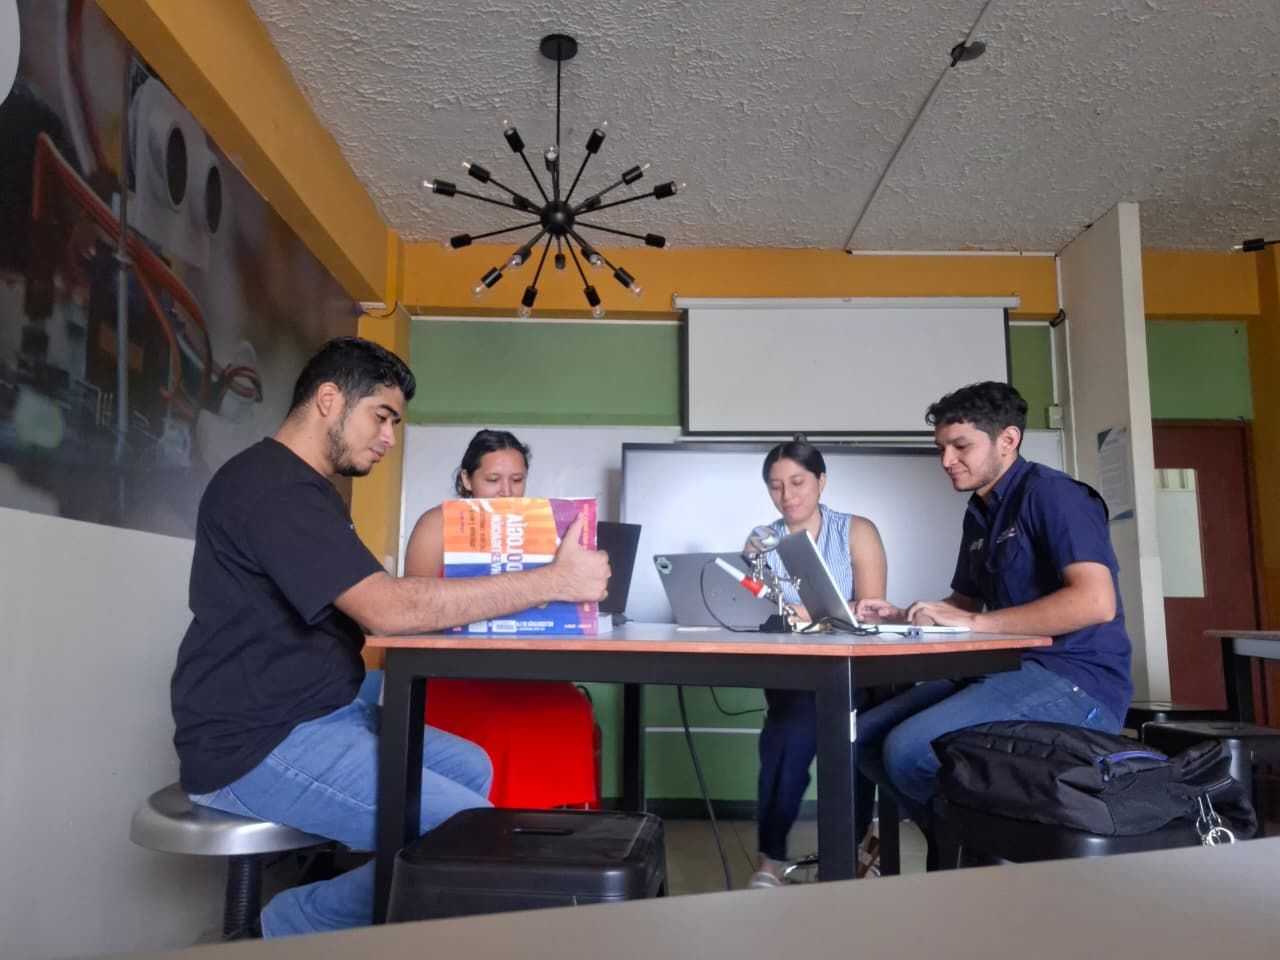
\includegraphics[width=0.8\textwidth]{assets/img/anexos/reunion-1/horizontal-1.jpeg}
    \caption{Reunión de lectura del libro \textit{Metodología de la investigación: las rutas cuantitativa, cualitativa y mixta} (Hernández Sampieri).}
    \label{fig:anexo1}
\end{figure}

\begin{figure}[h]
    \centering
    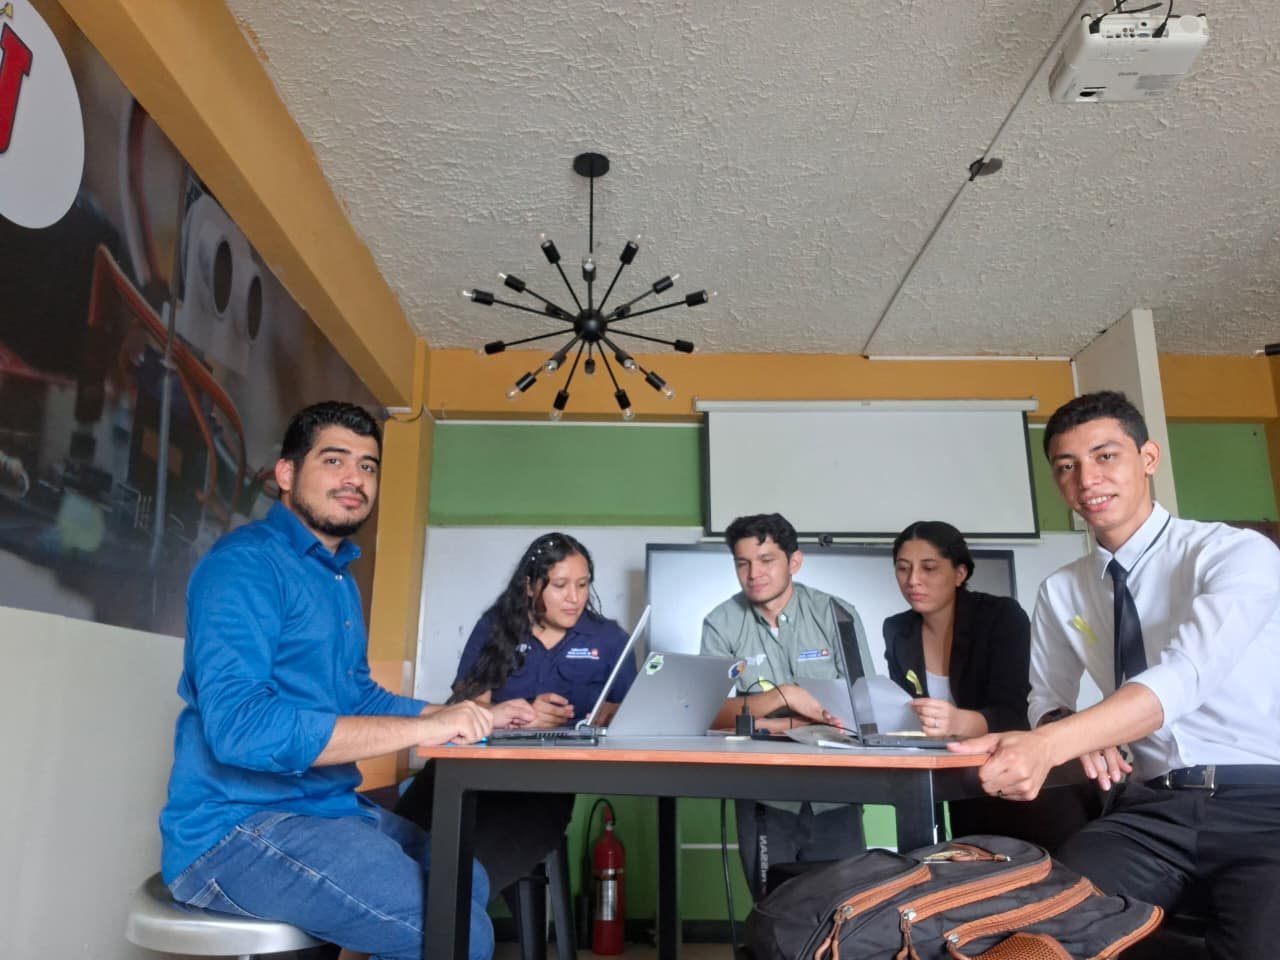
\includegraphics[width=0.8\textwidth]{assets/img/anexos/reunion-2/foto-2.jpeg}
    \caption{Reunión de trabajo para el desarrollo del Marco Teórico, Metodología y Análisis de Resultados.}
    \label{fig:anexo2}
\end{figure}

\end{document}
